% XCircuit output "tx_ltspice.tex" for LaTeX input from tx_ltspice.eps
\def\putbox#1#2#3#4{\makebox[0in][l]{\makebox[#1][l]{}\raisebox{\baselineskip}[0in][0in]{\raisebox{#2}[0in][0in]{\scalebox{#3}{#4}}}}}
\def\rightbox#1{\makebox[0in][r]{#1}}
\def\centbox#1{\makebox[0in]{#1}}
\def\topbox#1{\raisebox{-0.60\baselineskip}[0in][0in]{#1}}
\def\midbox#1{\raisebox{-0.20\baselineskip}[0in][0in]{#1}}
\begin{center}
\scalebox{0.4}{
\normalsize
\parbox{9in}{
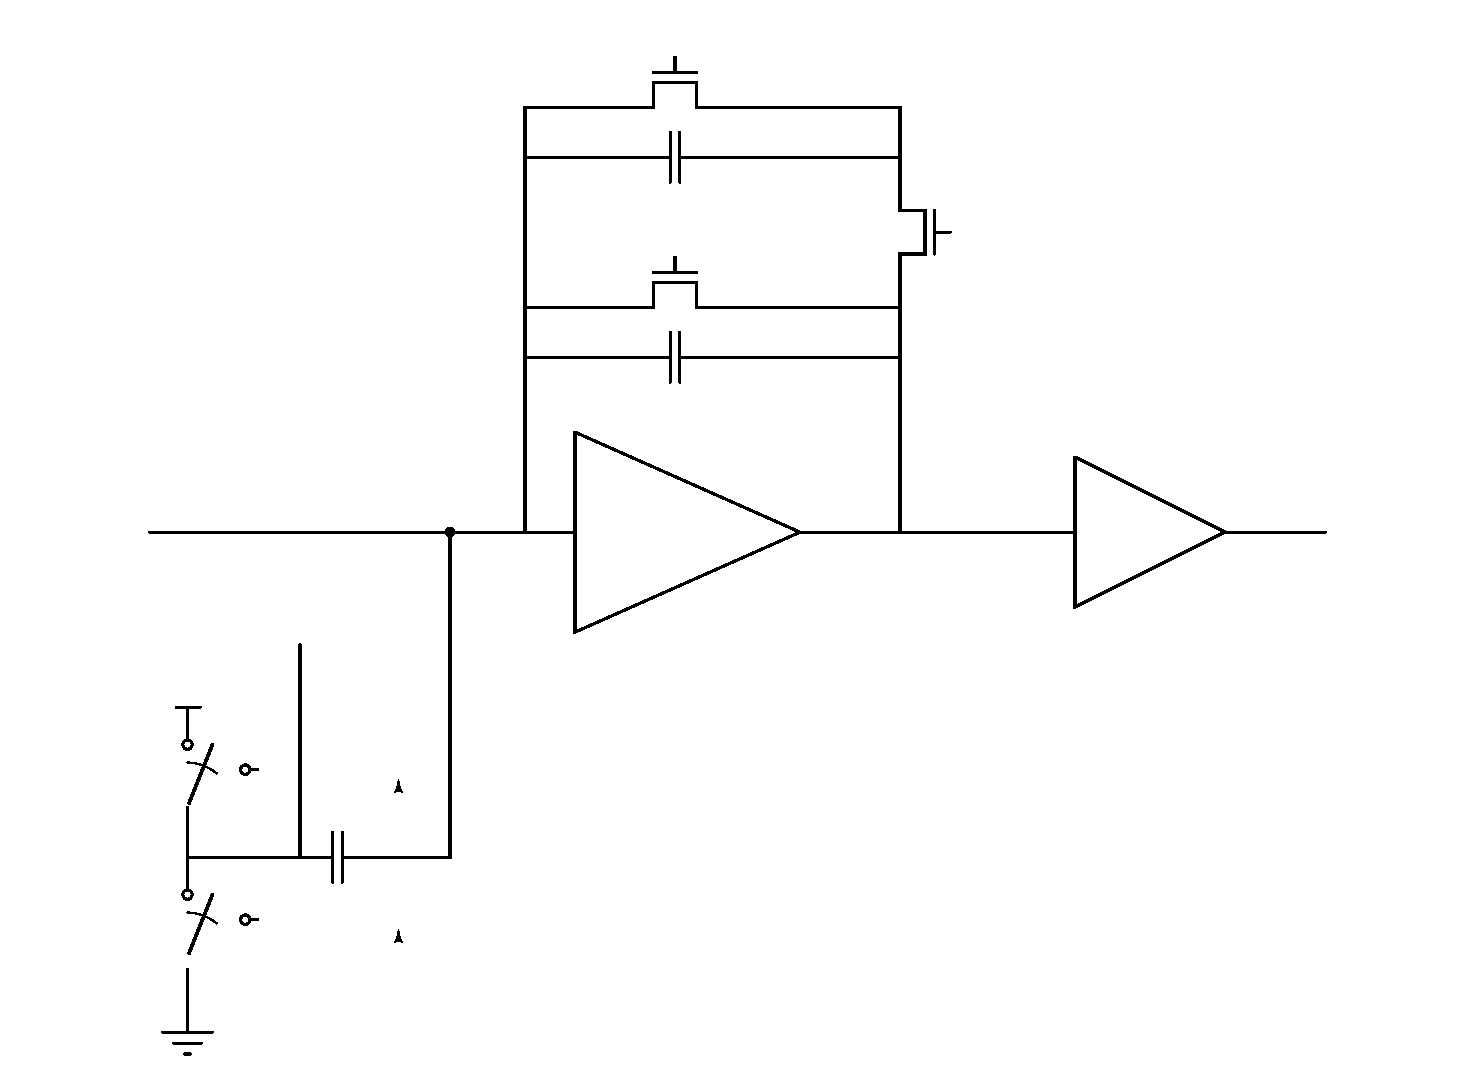
\includegraphics[scale=1]{./figures/theorical/csa_circuit2.eps}\\
% translate x=1152 y=860 scale 0.38
\putbox{0.22in}{3.62in}{1.2}{Vin\_csa}%
\putbox{0.72in}{2.45in}{1.2}{Vref\_pc}%
\putbox{1.56in}{2.87in}{1.2}{Cext\_pc}%
\putbox{4.06in}{5.54in}{1.2}{rst\_csa}%
\putbox{4.14in}{6.79in}{1.2}{rst\_csa}%
\putbox{6.39in}{5.54in}{1.2}{op\_mode}%
\putbox{8.72in}{3.62in}{1.2}{Vout\_csa}%
\putbox{0.14in}{1.87in}{1.2}{$\phi_1$\_pc}%
\putbox{0.06in}{1.04in}{1.2}{$\phi_2$\_pc}%
 } % close 'parbox'
 } % close 'scalebox'
\vspace{-\baselineskip} % this is not necessary, but looks better
\end{center}
